\documentclass[12pt, a4paper]{article}

\usepackage[T1, T2A]{fontenc}
\usepackage[utf8]{inputenc}
\usepackage[russian]{babel}
\usepackage{indentfirst}
\usepackage{graphicx}
\usepackage{xcolor}
\usepackage{titlesec}

\graphicspath{ {./images/} }

\setlength{\unitlength}{1cm}

\titleformat{\section}[block]
{\Large\normalfont\bfseries\filcenter}
{}{1em}{}

\titleformat{\subsection}[hang]
{\large\normalfont\bfseries\filcenter}
{}{1em}{}


\title{Изучение статистических закономерностей на примере
изучения фона космического излучения}
\author{Солодилов Михаил Б01-307}
\date{19.09.2023}

\begin{document}

\maketitle
\tableofcontents

\newpage

\section{Аннотация}

\textbf{Цель работы:} познакомиться с основными понятиями статистики,
на примере статистики регистрации фоновых космических частиц изучить
статистические закономерности однородного во времени случайного
процесса; проверить возможность описания исследуемого процесса
статистическими законами Пуассона и Гаусса; измерить среднее число
регистрируемых космических лучей в секунду и определить погрешность
результата.


\textbf{В работе используются:} счётчик Гейгера-Мюллера, компьютер
с интерфейсом для связи со счётчиком.


\section{Теоретические сведения}

\subsection{Излучение}
В любой физической лаборатории всегда присутствует радиоактивное
излучение. Источниками излучения являются космос и радиоактивные
вещества, в малых количествах содержащиеся всюду. Это излучение
называется радиоактивным фоном, а основную его часть всё-таки
составляют космические лучи.


В данной работе для регистрации
излучения используется счётчик Гейгера-Мюллера, который представляет
собой наполненный газом цилиндр с двумя электродами. Одним из
электродов является сам корпус. Вторым является тонкая нить,
натянутая вдоль оси корпуса. Необходимое напряжение подаётся на
электроды встроенным блоком питания. Частицы, попадая в счётчик,
ионизуют газ, получившиеся электроны лавиной ионизуют ещё больше
молекул газа, в следствие чего можно зафиксировать импульс тока,
что означает попадание частицы. 

Число зарегистрированных частиц зависит от времени измерения,
размеров счётчика, давления и состава газа, материалов, из которых
изготовлен счётчик.

\newpage

\subsection{Статистические понятия}

При любом физическом измерении полученные результат отличается
от некоторого истинного значения. Погрешности измерений складываются
из многих факторов, связанных с методикой измерения, неточностями
используемого оборудования и случайными погрешностями, которые
меняют свою величину и знак от опыта к опыту. Частным случаем случайных
ошибок являются статистические ошибки, вызываемые флуктуациями самой
измеряемой величины. В нашем эксперименте как раз есть такая флуктуирующая
величина - интенсивность космического излучения, причём флуктуации
настолько велики, что все остальные погрешности можно считать несущественными.


Пусть при некотором измерении за время $\tau = 10$ с зарегистрировано
$n$ космических частиц. Это совсем не значит, что за следующие 10 с
тоже зарегистрируется $n$ частиц. Поэтому для нас имеет значение среднее
количество зарегистрированных частиц. Если $n_1, n_2, n_3...$ - результаты
измерений, всего их $N$, то

\[\langle n \rangle \equiv \frac{1}{N}\sum_{i = 1}^{N}{n_i}.\]

Если продолжать проводить измерения, можно ожидать, что среднее будет
стремиться к некоторому конечному числу, которое можно назвать
\textit{"истинным"} средним значением числа регистрируемых частиц.
В математике такое число называется \textit{"математическим ожиданием"}.

\[\bar{n} = \lim_{n\to\infty} \langle n \rangle\]

Но число измерений всегда конечно, поэтому и среднее значение мы
можем измерить только с некоторой погрешностью.


Кроме среднего значения важно знать, насколько сильно флуктуируют
значения $n_i$ от опыта к опыту. Количественную меру флуктуаций принято
измерять среднеквадратичным отклонением(дисперсией) $\sigma_n$. По определению:
\[\sigma_n ^ 2 \equiv \frac{1}{N}\sum_{i = 1}^{N}{(n_i - \langle n \rangle) ^ 2}\]

Аналогично при $N\to\infty$ дисперсия стремится к некоторому предельному
\textit{"истинному"} значению:
\[\sigma ^ 2 = \lim_{N\to\infty}\sigma_n ^ 2\]


Из теории погрешностей известно, что дисперсия связана с погрешностью
среднего значения при независимых измерениях следующей формулой:

\[\sigma_{\langle n \rangle} = \frac{\sigma_n}{\sqrt{n}}.\]


\subsection{Гистограммы и вероятности}

\subsubsection*{Общее}

Среднее и дисперсия — это очень важные характеристики,
но не дающие \textit{полной} информации о флуктуирующей величине.
Более детальную информацию о ней можно получить, если собрать
\textit{статистику} того, как часто те или иные значения $n$ встречаются среди
многочисленных результатов опыта. Построим график, откладывая по оси абсцисс
число частиц, зарегистрированных при измерениях, а по оси ординат — долю
случаев (по отношению к общему числу измерений), в которых было зафиксировано
данное количество частиц. Например, если некоторое значение $n$ встретилось в
серии из $N$ измерений $N_n$ раз, то по вертикали отложим отрезок
высотой $w_n = \frac{N_n}{N}$. Построенный график содержит дискретно
расположенные точки, которые для наглядности обычно соединяются между собой,
изображая их в виде совокупности вертикальных прямоугольников.


В пределе $N\to\infty$ столбчатая гистограмма будет стремиться к некоторому
предельному состоянию. Предельные значения частот $w_n$ называют
\textit{вероятностями} соответствующих событий. Для вероятностей можно
строить различные теоретические модели, которые можно проверять на опыте,
сравнивая практические гистограммы со значениями, предсказанными
\textit{теорией вероятностей}.


При малых $N$ гистограмма может довольно сильно отличаться от теоретической.
По мере роста числа измерений $N$ пик гистограммы будет приближаться
к предельному среднему значению $\bar{n}$. Ширина гистограммы по порядку
величины совпадает со среднеквадратичным отклонением $\sigma_n$.
Если величина $n$ близка к $\bar{n}$, её вероятность будет максимальна.
А при удалении от $\bar{n}$ на расстояния, превышающие в несколько раз
$\sigma_n$, вероятность, как правило, быстро падает.


\subsubsection*{Пуассоновский процесс}

Если случайные события однородны во времени, а каждое последующее событие
никак не зависит от предыдущего, то последовательность таких событий
принято называть \textit{пуассоновским процессом}.


Для пуассоновского процесса может быть получено теоретическое распределение
вероятностей - \textit{распределение Пуассона}. Вероятности $w_n$ того,
что в эксперименте будет обнаружено $n$ частиц, для распределения
Пуассона имеют вид

\[w_n = \frac{\bar{n} ^ n}{n!}e^{-\bar{n}}.\]


Одним из наиболее характерных свойств этого распределения является
связь между его дисперсией и средним значением.

\[\sigma_n\approx\sqrt{\bar{n}}\]


\section{Методика измерений}

Измерений проводились с помощью счётчика Гейгера-Мюллера, подключённого
по USB к ноутбуку с необходимым программным обеспечением.

\subsection{Ход работы}

\begin{enumerate}
    \item Включить счётчик, запустить программу эксперимента.
    \item Через $4000$ с эксперимента сохранить данные, выданные программой.
\end{enumerate}

\section{Результаты измерений и обработка данных}

\subsection{Данные}

Программа выдала несколько графиков, а также текстовый файл, содержащий
количество зарегистрированных частиц за секунду.

\begin{center}
    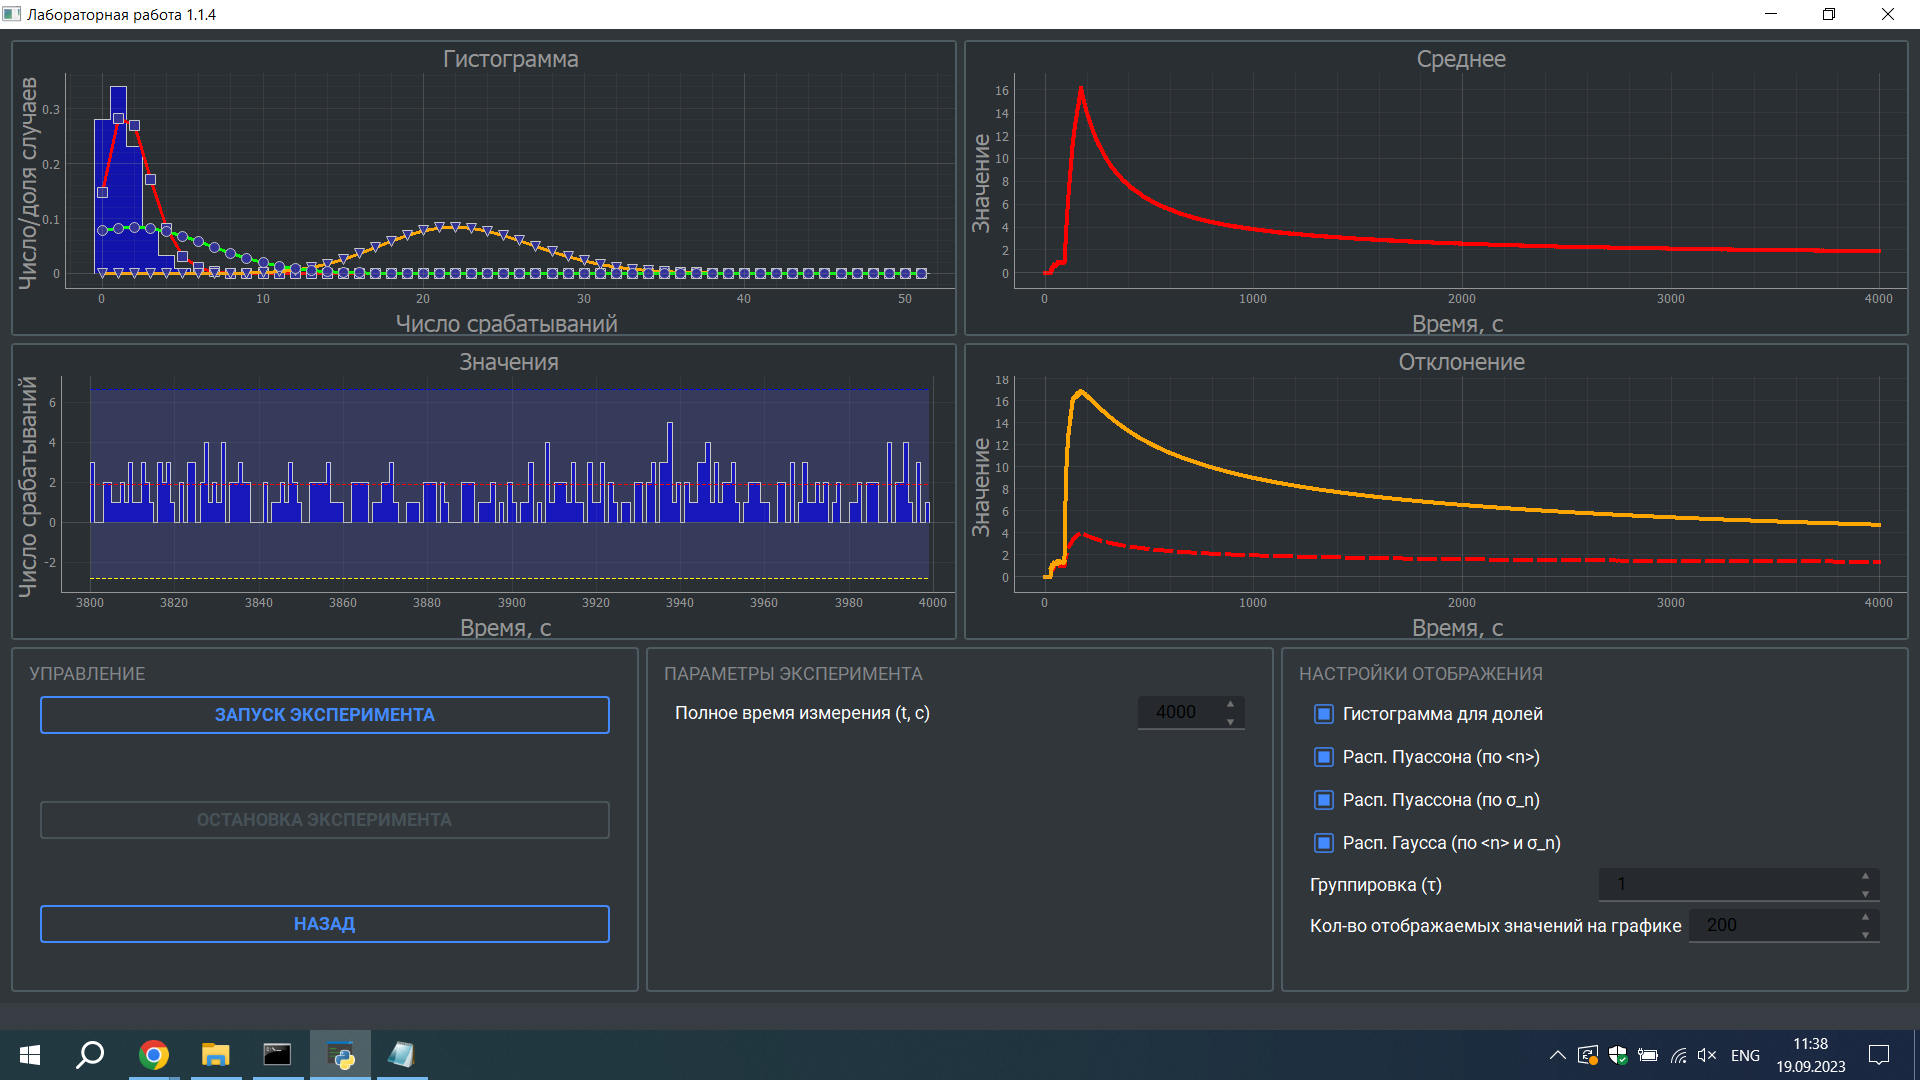
\includegraphics[width=\textwidth]{image}
\end{center}

Обработаем полученные данные, разбив их на промежутки длины
$\tau$.

\begin{center}
    Для $\tau = 10, 20, 30$ секунд рассчитаем следующие
    значения:
    \begin{itemize}
        \item $\langle n \rangle$ - среднее количество частиц.
        $\langle n \rangle = \frac{\sum_{i = 1}^{N} n_{i}}{N}$

        \item $\sigma_n$ - среднеквадратичное отклонение.
        $\sigma_n = \sqrt{\frac{1}{N}\sum_{i = 1}^{N}
        (n_{i} - \langle n \rangle)^2}$

        \item $i \cdot \sigma_n$ - попадание в $i\sigma_n$
        
        \item $\sigma_{\langle n \rangle}$ - погрешность $\langle n \rangle$.
        $\sigma_{\langle n \rangle} = \frac{\sigma_n}{\sqrt{n}}$

        \item $j$ - средняя интенсивность.
        $j = \frac{\langle n \rangle}{\tau}$

        \item $\sigma_j$ - погрешность средней интенсивности.
        $\sigma_j = \frac{\sigma_{\langle n \rangle}}{\tau}$
    \end{itemize}
\end{center}


\begin{center}
    \begin{tabular}{|c|c|c|c|}

        \hline
        
        & $\tau$ = 10s & $\tau$ = 20s & $\tau$ = 30s \\

        \hline

        $\langle n \rangle$ & 19.1 & 38.2 & 57.4 \\

        \hline

        $\sigma_n$ & 44.6 & 84.7 & 128.8 \\

        \hline

        $1 \cdot \sigma_n$ & 0.98 & 0.98 & 0.98 \\

        \hline

        $2 \cdot \sigma_n$ & 0.98 & 0.98 & 0.98 \\

        \hline

        $3 \cdot \sigma_n$ & 0.98 & 0.98 & 0.98 \\

        \hline

        $\sigma_{\langle n \rangle}$ &
        2.2 & 6.0 & 11.2 \\

        \hline

        $j, c^-1$ & 1.91 & 1.91 & 1.91 \\

        \hline

        $\sigma_j, c^-1$ & 0.22 & 0.30 & 0.37 \\

        \hline

    \end{tabular}
\end{center}

Можно сделать следующие выводы:

\begin{itemize}
    \item $\langle n \rangle$ - прямо пропорционально $\tau$, что очевидно.
    \item $\sigma_n$ - пропорционально $\tau$.
    \item $i \cdot \sigma_n$ - правило трёх сигм не соблюдается.
    \item $\sigma_{\langle n \rangle}$ - пропорционально $\tau$.
    \item $j$ - не зависит от $\tau$.
    \item $\sigma_j$ - пропорционально $\tau$.
\end{itemize}

\begin{center}
    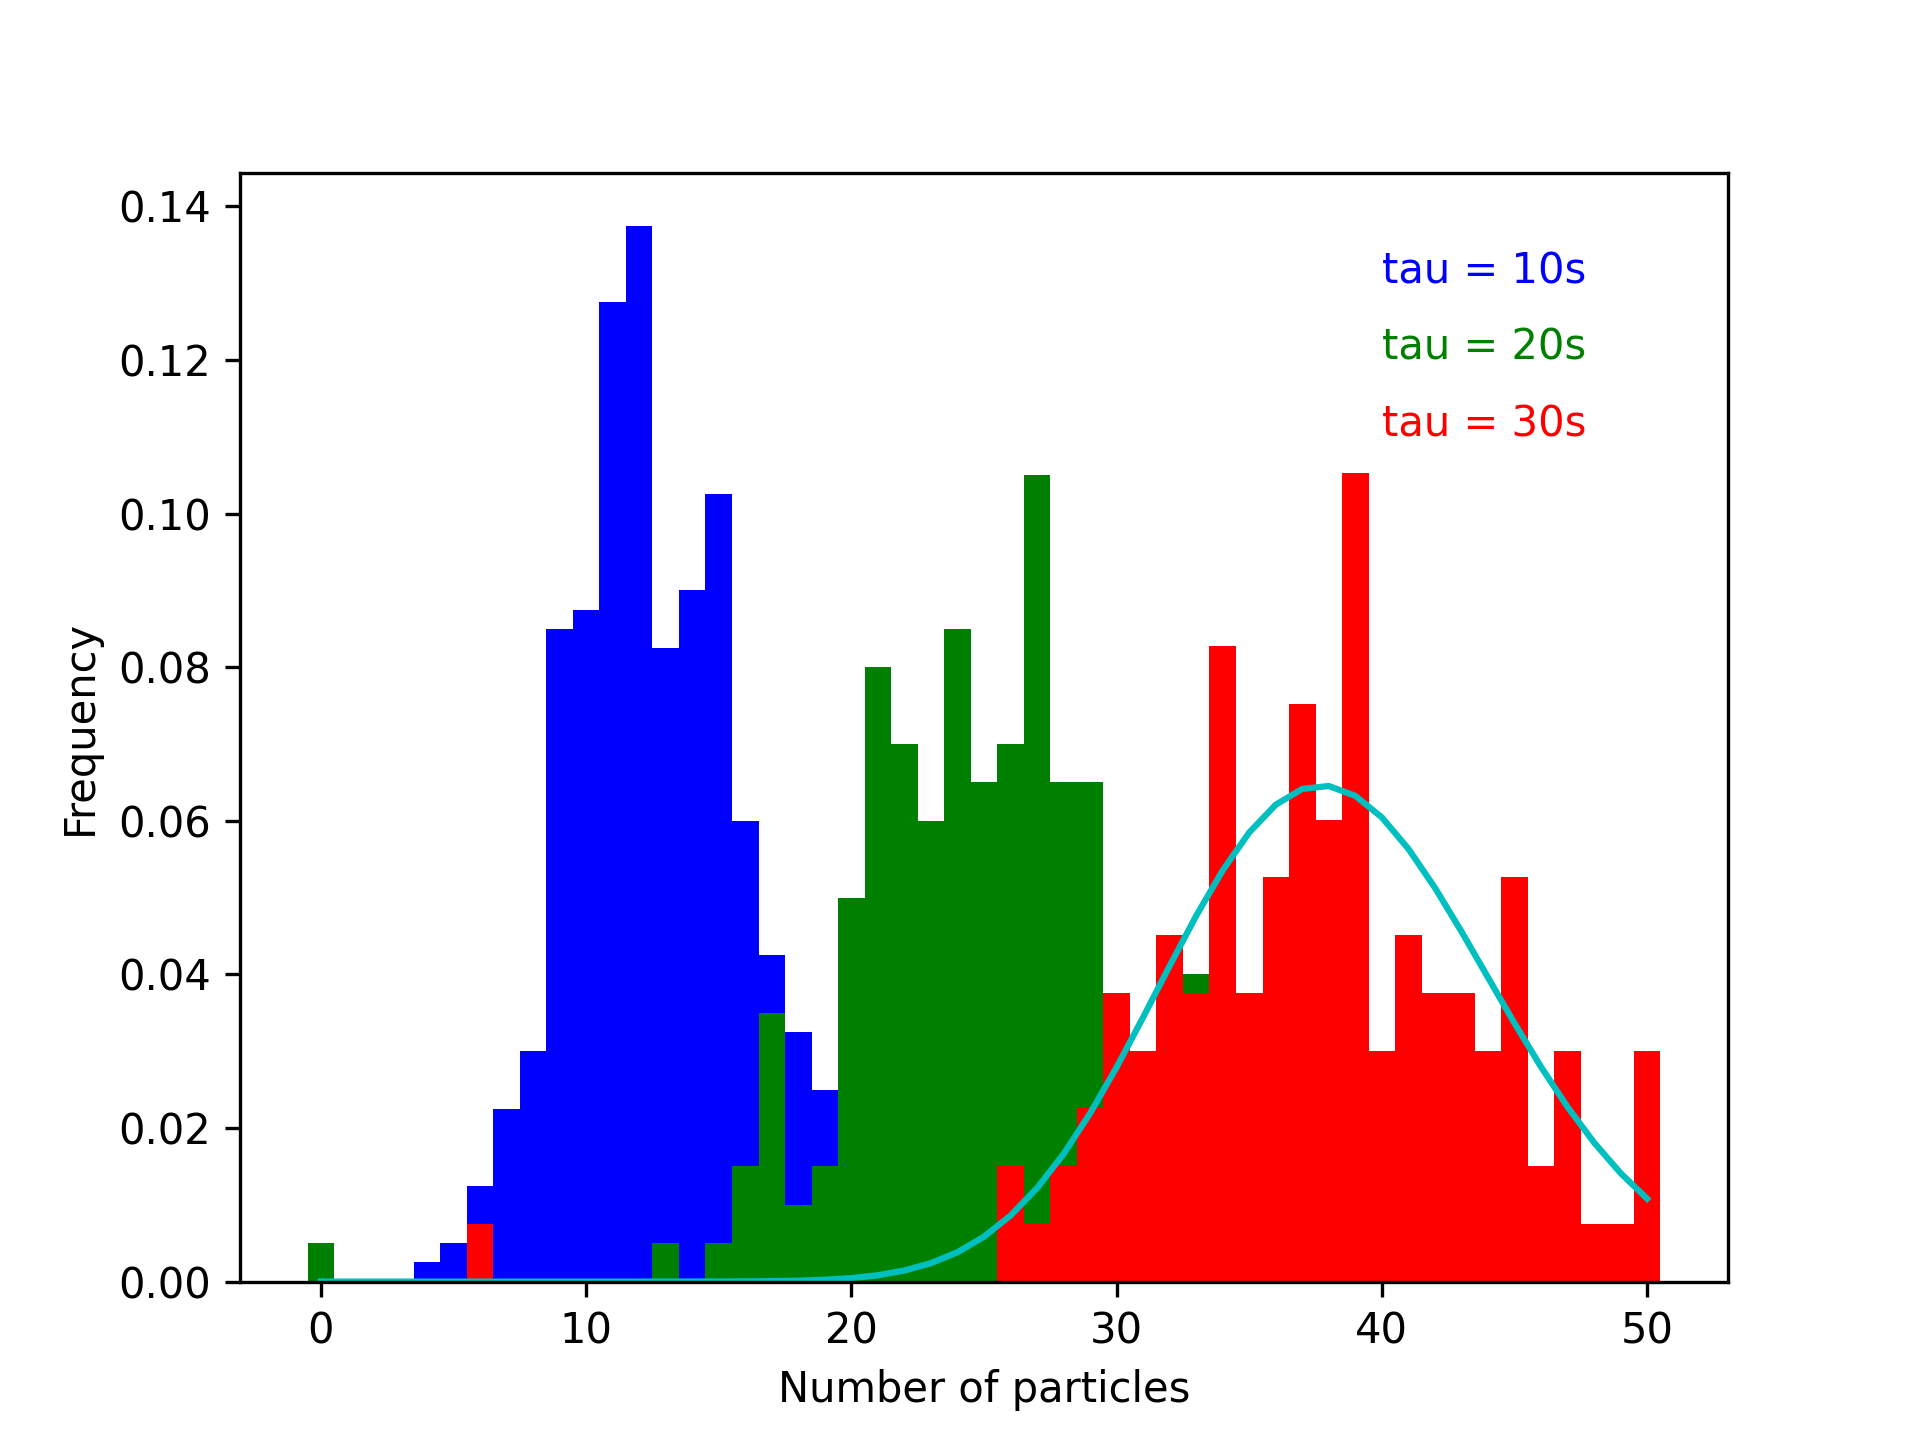
\includegraphics[width=\textwidth]{Figure bad}
\end{center}

Распределение Пуассона строилось для $\tau = 20$ с, однако, как мы видим,
оно вообще не ложится под настоящие данные.
При этом видно, что свойство распределения Пуассона
$\sigma_n \approx \sqrt{\langle n \rangle}$ здесь не работает.


При этом доли случаев, $|n - \langle n \rangle| < \sigma_n, 2\sigma_n,
3\sigma_n$ больше 0.97. Это вызвано огромным среднеквадратичным отклонением.
На это повлияли крайне сильные флуктуации, которые можно было наблюдать
на графиках в программе счётчика в начале эксперимента. Можно предположить,
что в некоторый момент эксперимента рядом с счётчиком находился источник
радиации.


В связи с этим я решил исключить данные, сильно выделяющиеся из массы.
Были получены следующие данные:

\begin{center}
    \begin{tabular}{|c|c|c|c|}

        \hline
        
        & $\tau$ = 10s & $\tau$ = 20s & $\tau$ = 30s \\

        \hline

        $\langle n \rangle$ & 12.7 & 25.4 & 38.1 \\

        \hline

        $\sigma_n$ & 3.5 & 5.4 & 6.4 \\

        \hline

        $1 \cdot \sigma_n$ & 0.68 & 0.65 & 0.70 \\

        \hline

        $2 \cdot \sigma_n$ & 0.95 & 0.97 & 0.95 \\

        \hline

        $3 \cdot \sigma_n$ & 0.99 & 0.99 & 0.99 \\

        \hline

        $\sigma_{\langle n \rangle}$ &
        0.18 & 0.39 & 0.56 \\

        \hline

        $j, c^-1$ & 1.27 & 1.27 & 1.27 \\

        \hline

        $\sigma_j, c^-1$ & 0.02 & 0.02 & 0.02 \\

        \hline

    \end{tabular}
\end{center}

По этим данным можно сказать:

\begin{itemize}
    \item $\langle n \rangle$ - прямо пропорционально $\tau$, что очевидно.
    \item $\sigma_n \approx \langle n \rangle$.
    \begin{center}
        \begin{tabular}{|c|c|c|c|}
            \hline
            & $\tau = 10$ с & $\tau = 20$ с & $\tau = 30$ с \\
            \hline
            $\sqrt{n}$ & 3.56 & 5.04 & 6.17 \\
            \hline
            $\sigma_n$ & 3.5 & 5.4 & 6.4 \\
            \hline
            $\varepsilon_{\sigma_n}$, \% & 1.71 & 6.67 & 3.59 \\ 
            \hline
        \end{tabular}
    \end{center}
    \item $i \cdot \sigma_n$ - правило трёх сигм соблюдается.
    \item $\sigma_{\langle n \rangle}$ - пропорционально $\tau$.
    \item $j$ - не зависит от $\tau$.
    \item $\sigma_j$ - не зависит от $\tau$.
\end{itemize}

\begin{center}
    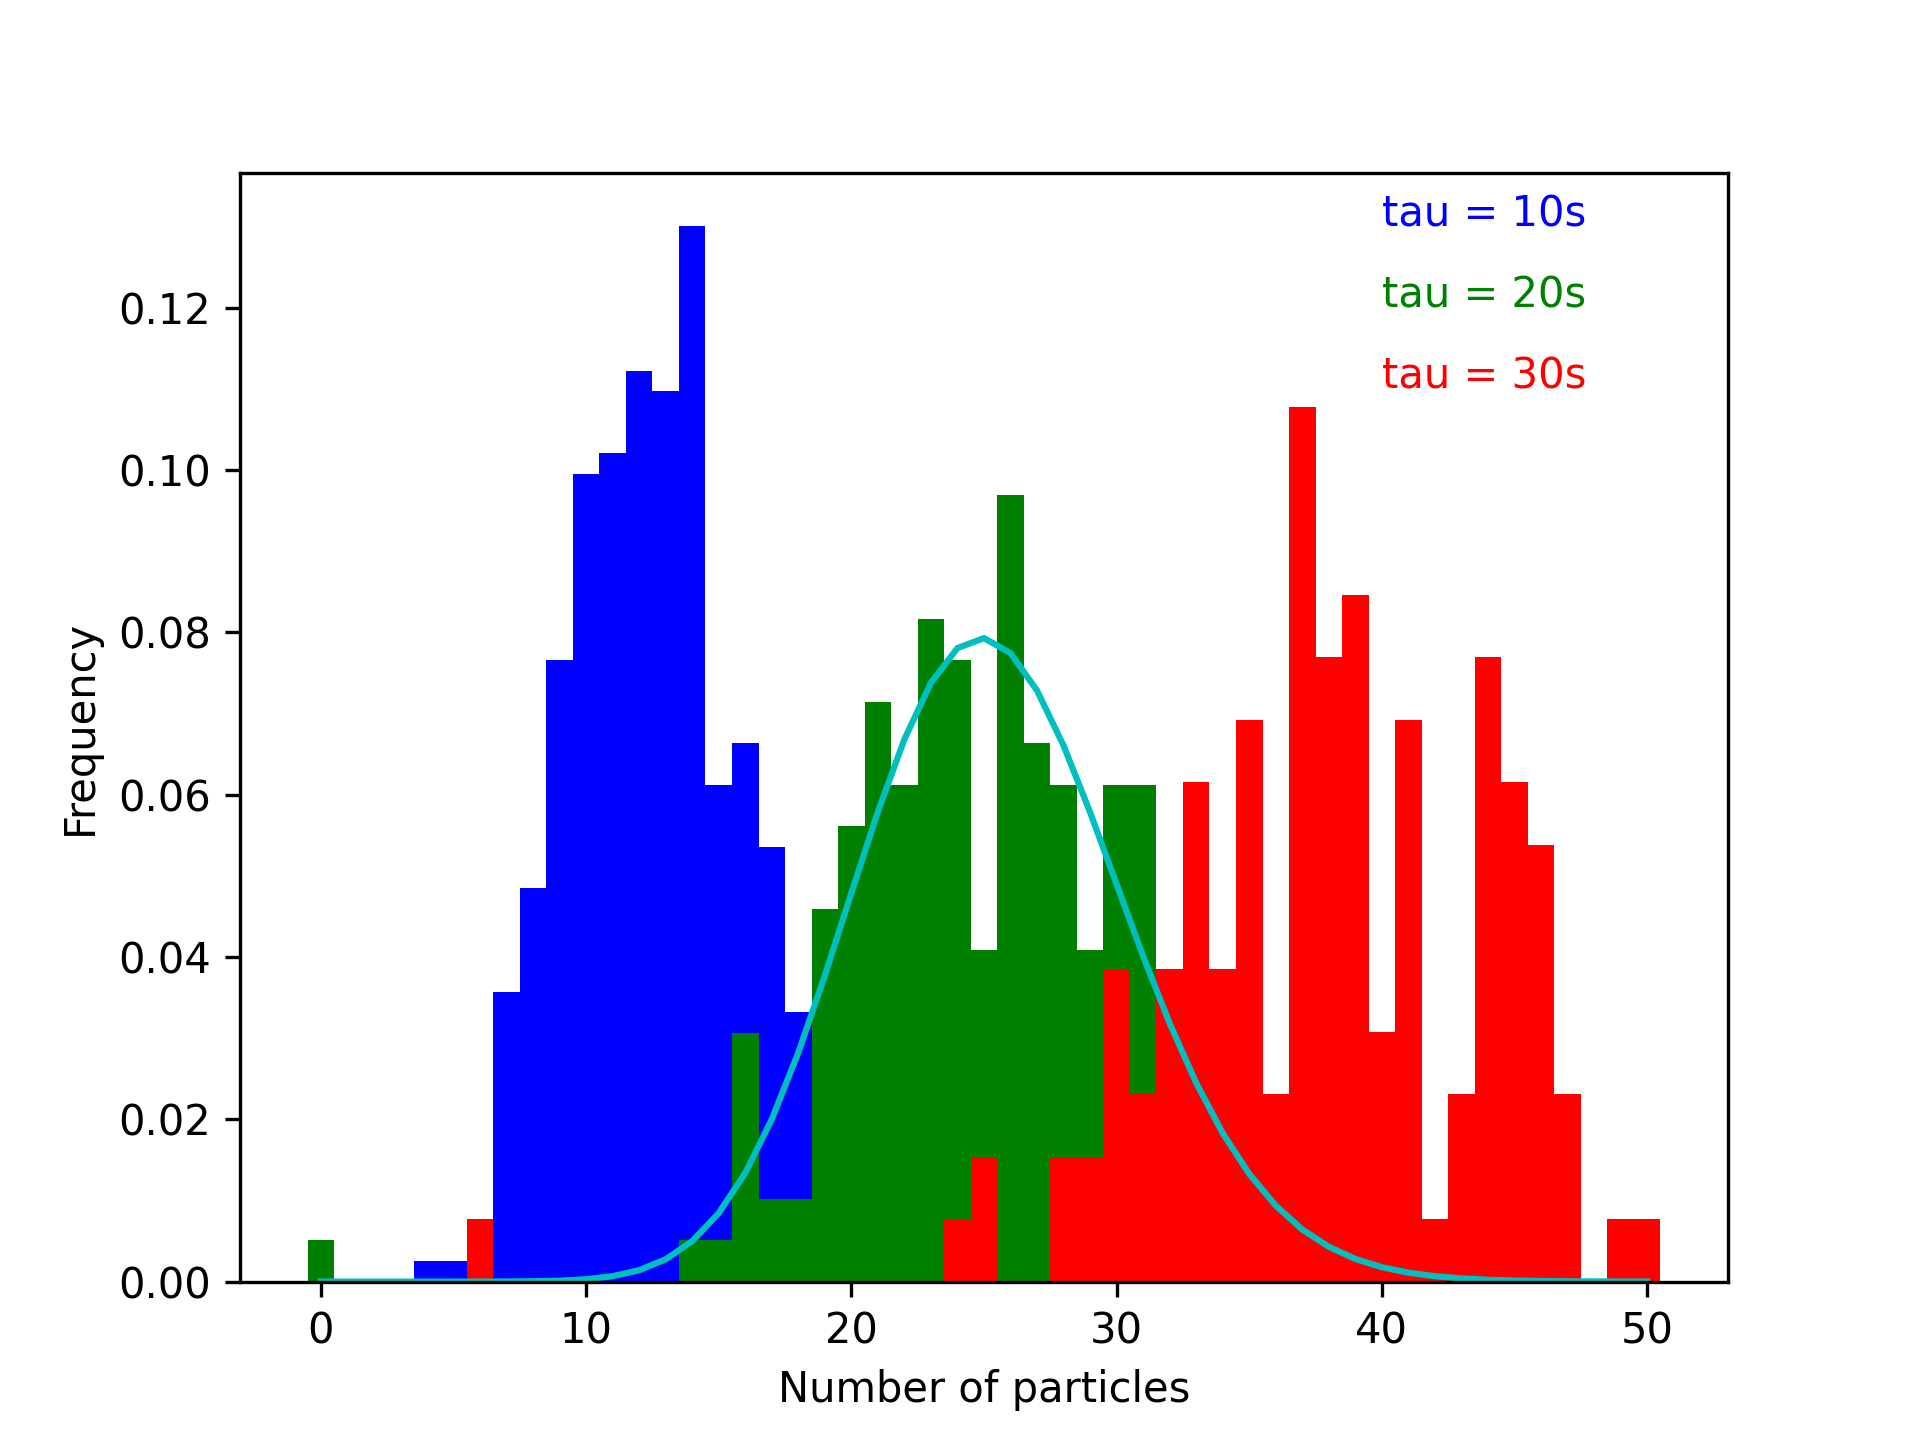
\includegraphics[width=\textwidth]{Figure good}
\end{center}

\subsection{Вывод}

График построен для $\tau = 20$ с, и он хорошо ложится на гистограмму.
В целом данные достаточно хорошо совпадают с теоретическими данными
(в пределах 7\%, говоря о $\sigma_n$), что говорит о случайном и независимом
характере космического излучения.

\end{document}